\documentclass[conference,a4paper]{IEEEtran}
% IEEEtran provides the IEEE layout: two columns, 10 pt Times, section headings
% ("I. INTRODUCTION", "A. Subsection"), "Fig." and "TABLE I" captions, and
% references to subsections printed as "Section III-A".
% Single-column variant: use \documentclass[conference,onecolumn,a4paper]{IEEEtran}
% and set \figwidth below to 0.62\columnwidth.

% ----------------------------------------------------------------- Fonts
\usepackage[T1]{fontenc}
\usepackage[utf8]{inputenc}
% Times text and math. newtx is preferred; mathptmx is a fallback that ships
% with every TeX distribution.
\IfFileExists{newtxtext.sty}
  {\usepackage{newtxtext}\usepackage{newtxmath}}
  {\usepackage{mathptmx}\usepackage{amssymb}}   % amssymb: \mathbb (newtxmath has it built in)
\usepackage{microtype}
% Long file names in \texttt cannot be hyphenated; allow a little extra
% inter-word space instead of letting them stick out into the margin.
\setlength{\emergencystretch}{2em}

% ---------------------------------------------------------------- Content tools
\usepackage{amsmath}
\interdisplaylinepenalty=2500   % recommended by IEEEtran when using amsmath
\usepackage{graphicx}
\usepackage{booktabs}
\usepackage{array}
\usepackage{enumitem}
\usepackage{listings}
\usepackage{xcolor}
\usepackage{balance}   % equal-height columns on the last page (IEEE style)

% Figures generated by assignment_3/plot_results.py --physical-cores 4. They are
% designed for a 3.5 in column, so \includegraphics[width=\columnwidth] prints
% them at the intended size (see common/plotting_style.md).
\graphicspath{{../results/}}
\newcommand{\figwidth}{\columnwidth}

% Code listings (small, monospaced, light frame). The listing is a float
% (float=t), so it is never split across columns or pages.
\lstset{basicstyle=\footnotesize\ttfamily, frame=lines, framesep=3pt,
        columns=fullflexible, keepspaces=true, xleftmargin=0pt, xrightmargin=0pt}

% Links in the deep blue used for omp_tiled in the figures.
\definecolor{linkblue}{HTML}{1F43B2}
\usepackage[colorlinks=true,linkcolor=linkblue,citecolor=linkblue,urlcolor=linkblue]{hyperref}
\hypersetup{pdftitle={Parallel Matrix Multiplication and Vectorisation},
            pdfauthor={Javier Ruano Hernández}}

% ------------------------------------------------------------- Placeholders
% \TODO{...} prints a red marker in the PDF so no placeholder is forgotten.
\newcommand{\TODO}[1]{\textcolor{red}{\textbf{[TODO: #1]}}}

% ------------------------------------------------------------------ Shortcuts
\newcommand{\bigO}[1]{\mathcal{O}\!\left(#1\right)}
\newcommand{\code}[1]{\texttt{#1}}
\newcommand{\seqk}{\code{seq\_tiled}}
\newcommand{\ompk}{\code{omp\_tiled}}
\newcommand{\simdk}{\code{omp\_simd\_tiled}}
\newcommand{\Tseq}{T_{\mathrm{seq}}}
\newcommand{\Sself}{S_{\mathrm{self}}}

% =============================================================================
\title{Parallel Matrix Multiplication\\and Vectorisation}
\author{\IEEEauthorblockN{{Javier Ruano Hernández}}
\IEEEauthorblockA{Big Data -- Assignment 3\\
Universidad de Las Palmas de Gran Canaria (ULPGC)\\
% Check that the repository is public (or that the instructor has access).
Code and data: \url{https://github.com/javierruanohdez/big-data-assignments/tree/main/assignment_3}}}

\begin{document}
\maketitle

% =============================================================================
% ABSTRACT
% =============================================================================
% All numbers in this report are computed from results/measurements.csv
% (135 runs) and match results/results_summary.md. Recompute them if you
% re-run the benchmark.
\begin{abstract}
We parallelise the cache-blocked (tiled) dense matrix multiplication of
Assignment~2 with OpenMP and add explicit SIMD vectorisation, in C. Three
kernels with identical arithmetic and bit-identical results, a sequential one,
a multithreaded one with a scalar inner loop and a multithreaded one with
\code{\#pragma omp simd}, were run for $n = 500$, 1000 and 2000 with $p = 1$,
2, 4 and 8 threads on a laptop CPU with 4 cores and 8 hardware threads, five
times per configuration. Vectorisation was switched on and off loop by loop and
verified from the compiler's report. At $n = 2000$, eight threads made the
scalar kernel 4.56 times faster than the sequential kernel (efficiency 57\%),
and threads plus SIMD 10.9 times (0.445~s), the product of 4.56 from threads
and 2.38 from SIMD. SIMD alone gave 3.75 with one thread, but its gain shrank
with more threads: relative to itself, the vector kernel reached 2.53 on eight
threads and the scalar kernel 3.99. Moving from 4 to 8 threads, onto SMT
siblings, gave 1.45 for the scalar and 1.06 for the vector kernel. Estimated
memory traffic rules out a DRAM bandwidth limit; the flattening is consistent
with resources shared within and between cores. With one thread, the OpenMP kernel
was 13--37\% \emph{faster} than the sequential one, so OpenMP's own overhead
stayed below what this experiment resolves. These results describe one machine
and one configuration.
\end{abstract}

\begin{IEEEkeywords}
matrix multiplication, OpenMP, shared-memory parallelism, SIMD, vectorisation,
speedup, parallel efficiency, simultaneous multithreading.
\end{IEEEkeywords}

% =============================================================================
\section{Introduction and Objective}
\label{sec:intro}
% =============================================================================

Assignment~2 made the dense matrix multiplication cache-friendly: loop
reordering and tiling cut the time at $n = 2000$ from 15.6 to about 3.5~s. It
left two resources unused. The kernels ran on one of the four cores of the
test machine, and their inner loop processed one double per instruction; the
report concluded that this scalar loop, not memory traffic, limited the tiled
kernel. This report attacks both limits on the same tiled kernel: shared-memory
multithreading with OpenMP~\cite{openmp52,chapman2008} distributes the work
over the cores, and SIMD vectorisation processes several doubles per
instruction~\cite{hennessy2017}.

\paragraph{Objective} We answer the following research question:

\begin{quote}
\emph{How does the time of the tiled matrix multiplication scale with the
number of threads, why does it depart from the ideal, and how much does
explicit SIMD vectorisation add on top of multithreading?}
\end{quote}

\begin{enumerate}[label=\textbf{RQ\arabic*.}, leftmargin=3.2em, itemsep=1pt]
  \item What does the OpenMP machinery cost with a single thread ($p = 1$)?
  \item How do speedup and efficiency evolve with $p$ and $n$, and where and
        why does scaling flatten?
  \item What happens when the threads exceed the physical cores and share
        them through simultaneous multithreading (SMT)?
  \item How much does SIMD add, and how do its gain and the threading gain
        combine?
\end{enumerate}

\paragraph{Contributions and scope} We provide (i)~three kernels in one program
that differ in exactly one aspect each, with bit-identical results;
(ii)~a build that forces the inner loop to be scalar or vector, verified from
the compiler's vectorisation report; (iii)~an automated pipeline that
validates, measures and analyses all configurations; and (iv)~a
measurement-based analysis that separates the threading and SIMD gains. Code
and raw data are in the repository linked on the first page. The results
describe one machine (Section~\ref{sec:environment}).

% =============================================================================
\section{Background and References}
\label{sec:background}
% =============================================================================

\subsection{Shared-Memory Parallelism with OpenMP}
In OpenMP's fork-join model, a program runs on one thread until it reaches a
parallel region, where a team of $p$ threads starts; the threads share one
address space~\cite{openmp52,chapman2008}. A \code{parallel for} construct
divides the iterations of a loop among the team and ends with an implicit
barrier, so the region lasts as long as its slowest thread. With
\code{schedule(static)} the iterations are split into equal contiguous chunks
before the loop starts; dynamic schedules hand out chunks at run time through
a shared counter. Parallel execution has three costs that a sequential program
does not pay: creating the threads (once per program in typical runtimes),
forking and joining the team and synchronising at barriers, which
microbenchmarks measure in microseconds~\cite{bull1999}, and load imbalance,
since equal chunks finish at different times on unequal cores.

\subsection{False Sharing}
Caches keep cores coherent at the granularity of a cache line, 64~bytes on
current x86-64 CPUs~\cite{hennessy2017,drepper2007}. When two cores write
different variables that lie in the same line, each write invalidates the
other core's copy, and the line bounces between their caches as if the data
were shared~\cite{torrellas1994}. A classic trap is an array of per-thread
counters updated in an inner loop. It is avoided by giving every thread a
disjoint region of output whose boundaries fall on cache-line boundaries, and
by keeping accumulators private.

\subsection{Speedup, Efficiency and Amdahl's Law}
Let $\Tseq$ be the time of the sequential program and $T_p$ the time with $p$
threads. Speedup and efficiency are
\begin{equation}
  S(p) = \frac{\Tseq}{T_p}, \qquad E(p) = \frac{S(p)}{p},
  \label{eq:speedup}
\end{equation}
with ideal values $S(p) = p$ and $E(p) = 1$. If a fraction $f$ of the work is
serial, Amdahl's law bounds the speedup~\cite{amdahl1967}:
\begin{equation}
  S(p) \le \frac{1}{f + (1 - f)/p}.
  \label{eq:amdahl}
\end{equation}
Gustafson observed that larger problems usually have a smaller serial
fraction, so they scale better~\cite{gustafson1988}. Inverting
\eqref{eq:amdahl} for a measured speedup gives the Karp--Flatt
metric~\cite{karp1990},
\begin{equation}
  e = \frac{1/S(p) - 1/p}{1 - 1/p},
  \label{eq:karpflatt}
\end{equation}
the serial fraction that would explain the measurement. It absorbs every loss,
not only serial code: overheads, imbalance and contention for shared hardware.
Finally, the roofline model~\cite{williams2009} relates performance to the
arithmetic intensity of a kernel (operations per byte moved from memory). A
$b \times b$ tile product performs $2b^3$ floating-point operations on two
input tiles of $8b^2$ bytes each, an intensity of $b/8$, i.e.\ 8 operations per
byte for $b = 64$: tiling turns matrix multiplication from a memory-bound into
a compute-bound kernel.

\subsection{SIMD Vectorisation}
SIMD instructions apply one operation to all lanes of a vector register:
4 doubles in a 256-bit AVX2 register, 8 in a 512-bit AVX-512
register~\cite{hennessy2017}. Register width and hardware throughput may
differ: the Zen~5 and Zen~5c cores of AMD's Strix Point mobile processors have
256-bit floating-point datapaths, half the width of an AVX-512
register~\cite{tpu2024}. The i-k-j inner loop
$c_{ij} \mathrel{+}= a_{ik} b_{kj}$ over $j$ suits SIMD perfectly: its
iterations are independent and access $B$ and $C$ with unit stride. Compilers
vectorise such loops automatically if they can prove that the iterations are
independent; when two pointers may overlap, they add a run-time overlap check
or keep the loop scalar. The OpenMP directive \code{\#pragma omp simd} asserts
independence and requests a vector loop~\cite{openmp52}. A vector loop is
followed by a short scalar or narrower \emph{epilogue} for the remaining
iterations. Because the lanes hold different output elements, vectorising over
$j$ does not change the order in which each $c_{ij}$ accumulates its terms,
unlike vectorising a sum.

\subsection{Simultaneous Multithreading and Oversubscription}
With SMT (Intel's Hyper-Threading), each core runs two hardware threads that
share its execution units, load/store units and private caches. SMT raises
throughput when one thread alone leaves resources idle, for example while
waiting for memory, and helps little when a thread already saturates a shared
resource~\cite{tullsen1995,hennessy2017}. \emph{Oversubscription} means more
software threads than hardware threads: the operating system must time-slice
them.

% =============================================================================
\section{Methodology}
\label{sec:method}
% =============================================================================

\subsection{Experimental Environment}
\label{sec:environment}
All measurements were taken on the machine described in
Table~\ref{tab:environment}, with other applications closed and the computer
connected to mains power. Its four cores are of two types, one Zen~5 core and
three Zen~5c cores with lower maximum clocks~\cite{nbc330}.

\begin{table}[t]
  \centering
  \caption{Hardware and software environment}
  \label{tab:environment}
  \footnotesize
  % Sources: lscpu, nproc, free, /etc/os-release, uname, gcc --version,
  % python3 --version, pip show. lscpu reports cache totals over the 4 cores.
  % Clock and core types: CPU specification (lscpu under WSL does not report
  % them); same CPU as in Assignments 1 and 2. Vector width: GCC's report.
  % Check the pandas/Matplotlib versions with: pip show pandas matplotlib
  \begin{tabular}{@{}l>{\raggedright\arraybackslash}p{0.64\columnwidth}@{}}
    \toprule
    \textbf{Item} & \textbf{Value} \\
    \midrule
    CPU model               & AMD Ryzen AI 5 330 w/ Radeon 820M \\
    Cores / logical threads & 4 cores (1 Zen~5 + 3 Zen~5c) / 8 threads (2-way SMT) \\
    Clock                   & 2.0~GHz base; boost up to 4.5~GHz (Zen~5 core)
                              and 3.4~GHz (Zen~5c cores) \\
    Caches                  & L1d 192~KiB, L1i 128~KiB, L2 4~MiB (i.e.\ 48~KiB,
                              32~KiB and 1~MiB per core); L3 8~MiB shared \\
    SIMD                    & AVX2 and AVX-512; GCC used 64-byte (512-bit) vectors \\
    RAM                     & 15~GiB (available to WSL~2) \\
    Operating system        & Ubuntu 26.04 LTS on WSL2 (Windows Subsystem for Linux) \\
    Kernel                  & 6.18.33.2-microsoft-standard-WSL2 \\
    C compiler / OpenMP     & GCC 15.2.0 with its OpenMP runtime (libgomp) \\
    Python                  & CPython 3.14.4 \\
    Analysis                & pandas 3.0.3, Matplotlib 3.10.9 \\
    \bottomrule
  \end{tabular}
\end{table}

\subsection{Implementations}
\label{sec:impl}
One C file, \code{parallel\_mult.c}, contains three kernels; all use 64-bit
doubles, flat row-major arrays, and the input loader and timer of the previous
assignments.

\paragraph{\seqk} The tiled kernel of Assignment~2 ($b = 64$; tile loops
$ii$-$jj$-$kk$ with i-k-j inside), unchanged except for one directive on its
innermost loop (see below). It is the sequential baseline.

\paragraph{\ompk} The same loops, with
\code{\#pragma omp parallel for schedule(static)} on the outermost tile loop
(Listing~\ref{lst:omp}). One iteration of $ii$ computes a whole block-row of
$C$ (64 rows, all columns, all $kk$), so different threads never write the
same element: no data races, no locks, atomics or reductions, and every
$c_{ij}$ still receives its terms in increasing $k$. Parallelising the $kk$
loop instead would make threads add into the same tile of $C$ concurrently.
The static schedule gives each thread a contiguous chunk of row tiles at no
run-time cost; since full tiles cost the same, it is balanced up to the
partial last tile: the largest share exceeds the mean by 2.4\% for every
measured $n$ and $p > 1$. \code{default(none)} forces every shared variable to
be declared, so none can be shared by accident. Each thread clears its own
block-row of $C$ immediately before accumulating into it, rather than clearing
all of $C$ serially, which would add a serial part to the timed region.

\paragraph{False sharing} The only shared data written is $C$, and there are
no shared counters or accumulators. Thread boundaries lie at rows that are
multiples of $b$, at byte offset $8bn\,r$ for an integer $r$. $C$ is allocated
64-byte aligned (\code{aligned\_alloc}), so with $b = 64$ every boundary is a
cache-line boundary and no line is ever written by two threads, for any $n$.

\paragraph{\simdk} \ompk{} with one change: \code{\#pragma omp simd} instead
of \code{\#pragma GCC novector} on the innermost loop (Listing~\ref{lst:omp}).
The assertion of independence holds, since $B$ and $C$ are separate arrays and
iteration $j$ updates only $c_{ij}$; it lets GCC emit the vector loop without
a run-time overlap check.

\begin{lstlisting}[language=C, float=t, caption={\simdk{} (simplified). \ompk{} is identical except for the inner-loop directive; \seqk{} has neither the outer pragma nor the per-block clearing.}, label=lst:omp, captionpos=b]
#pragma omp parallel for schedule(static) \
        default(none) shared(a, b, c, n, bs)
for (ii = 0; ii < n; ii += bs) {
 memset(&c[ii*n], 0, rows(ii)*n*8); /* own rows */
 for (jj = 0; jj < n; jj += bs)
  for (kk = 0; kk < n; kk += bs)
   for (i = ii; i < min(ii+bs, n); i++)
    for (k = kk; k < min(kk+bs, n); k++) {
     a_ik = a[i*n + k];
     #pragma omp simd  /* omp_tiled: novector */
     for (j = jj; j < min(jj+bs, n); j++)
      c[i*n + j] += a_ik * b[k*n + j];
    }
}
\end{lstlisting}

\paragraph{Forcing scalar and vector loops} All kernels are compiled with
\code{-O3 -march=native}, and at \code{-O3} GCC auto-vectorises the i-k-j inner
loop of \emph{every} kernel. The comparison of \ompk{} with \simdk{} would then
compare vector code with vector code. The two reference kernels therefore mark
their inner loop \code{\#pragma GCC novector} (GCC~14 and later), which keeps
that loop scalar while \code{-O3} still optimises it in every other way; the
program refuses to compile with older versions, which would ignore the
directive. In addition, \code{-std=c11} implies \code{-ffp-contract=off}: no
multiply and add is fused into one FMA instruction, so the scalar and vector
kernels round identically.

\paragraph{Thread control} The program disables dynamic adjustment of the
team size with \code{omp\_set\_dynamic(0)} and sets it from its
\code{--threads} argument with \code{omp\_set\_num\_threads}, which
overrides \code{OMP\_NUM\_THREADS}. It checks before timing that the team
really has $p$ threads; it prints the team size, and the harness records any
mismatch as an error. Most OpenMP runtimes, including libgomp, create their
threads at the first parallel region. In our program this is an untimed
region that fills $C$ with NaN using the same $p$; it also maps every page of
$C$ before the timer starts and exposes any element a kernel fails to write.
The timed kernel thus reuses a running team, and the comparison of \ompk{} at
$p = 1$ with \seqk{} measures the per-call cost of OpenMP (fork, join, schedule
computation), not thread creation.

\subsection{Inputs and Experimental Design}
\label{sec:design}
Inputs are the shared binary files of the previous assignments
(\code{common/\allowbreak data\_\allowbreak generator.py}): $n$, followed by
$A$ and $B$ as little-endian doubles drawn uniformly from $[-1, 1)$ with a seed
derived from 42 and $n$. Table~\ref{tab:parameters} lists the parameters. At
$n = 500$ the three matrices (5.7~MB) fit in the 8~MB L3 cache; at $n = 1000$
and 2000 (22.9 and 91.6~MB) they do not. The thread counts double from 1 to the
8 logical CPUs; $p = 16$ was configured but skipped by the harness, which never
runs more threads than logical CPUs. With \code{OMP\_PLACES=cores} and
\code{OMP\_PROC\_BIND=spread}, threads are pinned to cores and spread over
them: for $p \le 4$ each thread has its own core, and $p = 8$ places two
threads on every core. \seqk{} runs only with $p = 1$.

\begin{table}[t]
  \centering
  \caption{Fixed experimental parameters}
  \label{tab:parameters}
  \footnotesize
  \begin{tabular}{@{}l>{\raggedright\arraybackslash}p{0.70\columnwidth}@{}}
    \toprule
    \textbf{Parameter} & \textbf{Value} \\
    \midrule
    Sizes       & $n$ = 500, 1000, 2000 (dense) \\
    Kernels     & \seqk{} ($p = 1$), \ompk, \simdk; tile edge $b = 64$ \\
    Threads     & $p$ = 1, 2, 4, 8 ($p = 16$ skipped: more than the 8 logical CPUs) \\
    Repetitions & 5 per configuration, each in a fresh process; 300 s budget per run \\
    Inputs      & uniform in $[-1,1)$, base seed 42, shared binary files \\
    Compiler    & \code{gcc -O3 -march=native -ftree-vectorize -fopenmp -std=c11 -Wall -Wextra}
                  (all kernels) \\
    OpenMP      & \code{OMP\_PLACES=cores}, \code{OMP\_PROC\_BIND=spread};
                  dynamic adjustment off \\
    Timer       & \code{clock\_gettime(CLOCK\_MONOTONIC)}, ns resolution \\
    Memory      & peak RSS (GNU \code{time -v}) \\
    \bottomrule
  \end{tabular}
\end{table}

\subsection{Measurement Protocol}
The program times only the kernel call, with \code{CLOCK\_MONOTONIC}; this is
wall-clock time, which a speedup requires (CPU-time clocks add up the time of
all threads). Input loading, allocation, the NaN pre-fill, thread creation and
process start-up are excluded. A harness (\code{run\_benchmark.py}) runs every
repetition in a fresh process and records the peak resident set size (RSS)
with GNU \code{time -v}. Runs exceeding the 300-s budget are recorded as
timeouts. Since all kernels and thread counts produce bit-identical results, a
run whose checksum differs from the first one recorded for its input file
would be flagged as a mismatch and excluded.

\subsection{Metrics}
$S(p)$ and $E(p)$ follow \eqref{eq:speedup}, with $\Tseq(n)$ the median time
of \seqk{} and $T_p(n)$ the median time of the kernel with $p$ threads at the
same $n$. Because \seqk{} is scalar, $S(p)$ of \simdk{} contains both the
threading and the SIMD gain. Two further metrics separate them: the
\emph{self-relative speedup} $\Sself(p) = T(1)/T(p)$ of each kernel against
itself on one thread, and the \emph{SIMD gain}
$G(p) = T_{\mathrm{omp}}(p)/T_{\mathrm{simd}}(p)$ at equal $p$. They combine
exactly as
\begin{equation}
  S_{\mathrm{simd}}(p) = \frac{\Tseq}{T_{\mathrm{simd}}(p)}
                       = S_{\mathrm{omp}}(p)\cdot G(p).
  \label{eq:decomposition}
\end{equation}
We report medians and interquartile ranges (IQR $= Q_3 - Q_1$) over the five
repetitions~\cite{georges2007,kalibera2013}; speedups are ratios of medians.
The bands in Figs.~\ref{fig:speedup} and~\ref{fig:efficiency} run from
$\Tseq/Q_3(T_p)$ to $\Tseq/Q_1(T_p)$, the spread of the parallel runs. All
statistics and figures are produced by \code{plot\_results.py} from the raw
data.

\subsection{Validation}
% Numbers from verify_correctness.py; check them against your own console output.
Before benchmarking, \code{verify\_correctness.py} runs every kernel on six
cases: $A \times I$, $A \times 0$, a hand-computed $3 \times 3$ product, and
random inputs with $n = 10$, 100 and 131 (full and partial edge tiles; with
$n = 131$ every tile edge is uneven). Each case runs with $b = 64$ and $b = 7$
(many tiles per thread, and inner loops shorter than and not a multiple of the
vector width, so the epilogue runs), and the OpenMP kernels with 1, 2, 3, 4, 8
and 16 threads (uneven splits and, for small $n$, threads without work). Since
IEEE~754 addition is not associative~\cite{ieee754}, each result is compared
with a correctly rounded \code{math.fsum} reference using the tolerances of
the previous assignments, derived from the dot-product error
bound~\cite{higham2002}: an element passes if
\begin{equation}
  |x - x_{\text{ref}}| \le \tau_{\text{abs}} + \tau_{\text{rel}}\, |x_{\text{ref}}|,
\end{equation}
with $\tau_{\text{rel}} = 10^{-12}$, $\tau_{\text{abs}} = 100\, n^2 u$ and
$u = 2^{-53}$. All 156 runs passed: the identity, zero and $3 \times 3$ cases
were reproduced exactly, the largest error was $1.1 \times 10^{-14}$ (random
cases, $n = 100$ and 131), four orders of magnitude below $\tau_{\text{abs}}$,
and every result was bit-identical to that of \seqk. The script also parses
GCC's vectorisation report (\code{-fopt-info-vec-optimized}) and maps each
vectorised loop to its function. The report lists the inner loop of \simdk{}
as ``loop vectorized using 64 byte vectors'', with a 32-byte epilogue, and no
vectorised loop in \seqk{} or \ompk.

% =============================================================================
\section{Results}
\label{sec:results}
% =============================================================================

All 135 runs (3 sizes, 5 repetitions, 9 kernel and thread combinations)
completed within the time budget, with no timeouts, errors or checksum
mismatches. Throughout, 1~MB $= 2^{20}$ bytes.

\subsection{Execution Time}
\label{sec:res-time}

\begin{figure}[t]
  \centering
  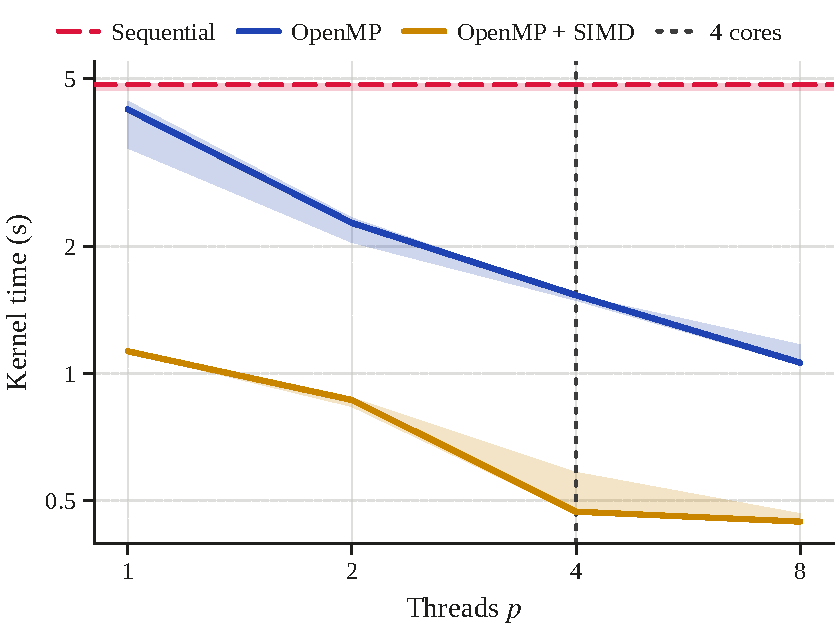
\includegraphics[width=\figwidth]{time_vs_threads.pdf}
  \caption{Median kernel time over five runs vs.\ threads $p$ at $n = 2000$
           (log-log), with interquartile-range bands. Dashed horizontal line:
           \seqk{} with its IQR. Dotted vertical line: the 4 physical cores;
           $p = 8$ uses SMT.}
  \label{fig:time}
\end{figure}

\begin{table}[t]
  \centering
  \caption{Results at $n = 2000$: median and IQR of the kernel time over five
           runs, speedup and efficiency over \seqk, and self-relative speedup}
  \label{tab:n2000}
  \footnotesize
  \setlength{\tabcolsep}{4.2pt}
  % Values computed from results/measurements.csv (same statistics as results_summary.md).
  \begin{tabular}{@{}lrrrrrr@{}}
    \toprule
    & & \multicolumn{2}{c}{\textbf{Time (s)}} & & & \\
    \cmidrule(lr){3-4}
    Kernel & $p$ & Median & IQR & $S(p)$ & $E(p)$ & $\Sself(p)$ \\
    \midrule
    \seqk  & 1 & 4.839  & 0.18  & 1.00  & 100\% & -- \\
    \midrule
    \ompk  & 1 & 4.227  & 1.00  & 1.14  & 114\% & 1.00 \\
           & 2 & 2.274  & 0.29  & 2.13  & 106\% & 1.86 \\
           & 4 & 1.532  & 0.043 & 3.16  & 79\%  & 2.76 \\
           & 8 & 1.060  & 0.12  & 4.56  & 57\%  & 3.99 \\
    \midrule
    \simdk & 1 & 1.128  & 0.011 & 4.29  & 429\% & 1.00 \\
           & 2 & 0.8648 & 0.041 & 5.59  & 280\% & 1.30 \\
           & 4 & 0.4701 & 0.12  & 10.29 & 257\% & 2.40 \\
           & 8 & 0.4451 & 0.020 & 10.87 & 136\% & 2.53 \\
    \bottomrule
  \end{tabular}
\end{table}

At $n = 2000$, \seqk{} takes 4.84~s (Fig.~\ref{fig:time},
Table~\ref{tab:n2000}). \ompk{} falls from 4.23~s with one thread to 2.27,
1.53 and 1.06~s with 2, 4 and 8 threads. \simdk{} takes 1.13~s with one thread,
less than \ompk{} with four, and falls to 0.865, 0.470 and 0.445~s. Per
multiply-add, \seqk{} costs 0.55--0.60~ns at every size, and \simdk{} on one
thread 0.14~ns at $n = 1000$ and 2000. The fastest configuration, \simdk{} with eight threads at
$n = 2000$, reaches 35.9~GFLOP/s.

With one thread, \ompk{} was faster than \seqk{} at every size: by 36.8\% at
$n = 500$ (46.2 vs.\ 73.1~ms), 24.8\% at $n = 1000$ (0.410 vs.\ 0.545~s) and
12.6\% at $n = 2000$ (4.23 vs.\ 4.84~s). At $n = 500$ and 1000 the ranges of
the five runs do not overlap (e.g.\ 43.9--51.4 against 71.5--80.6~ms at
$n = 500$); at $n = 2000$ they do (3.18--4.62 against 4.16--5.10~s), and the
five \ompk{} runs with $p = 1$ form two groups, 3.18--3.42~s and 4.23--4.62~s.
Most IQRs are below 15\% of the median; the largest are 32\% (\ompk, $n = 1000$,
$p = 2$), 25\% (\simdk, $n = 2000$, $p = 4$) and 24\% (\ompk, $n = 2000$,
$p = 1$).

The peak RSS did not grow with $p$: it stayed within 93.2--93.9~MB at
$n = 2000$, at most 3\% above the 91.6~MB of the three matrices, and varied by
less than 0.9~MB at every size. Threads add no measurable memory.

\subsection{Speedup and Efficiency}
\label{sec:res-speedup}

\begin{figure}[t]
  \centering
  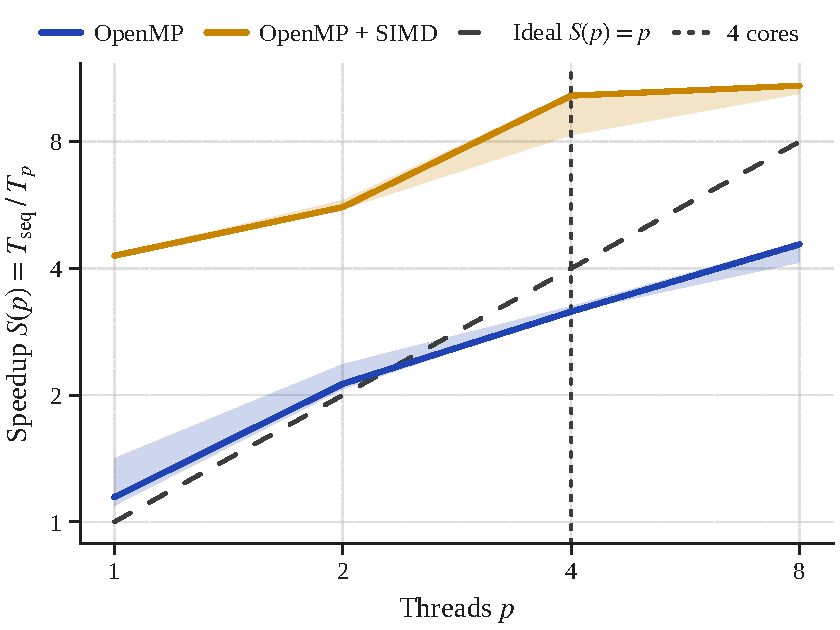
\includegraphics[width=\figwidth]{speedup_vs_threads.pdf}
  \caption{Speedup $S(p) = \Tseq/T_p$ vs.\ $p$ at $n = 2000$ (log-log), with
           the ideal $S(p) = p$ (dashed). \simdk{} includes the SIMD gain,
           since \seqk{} is scalar. Bands: $\Tseq/Q_3(T_p)$ to $\Tseq/Q_1(T_p)$.}
  \label{fig:speedup}
\end{figure}

\begin{figure}[t]
  \centering
  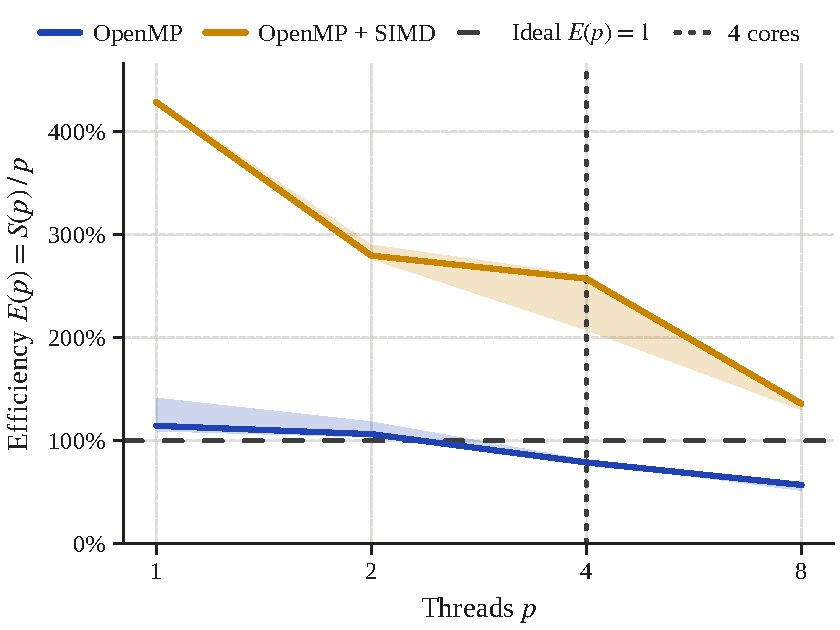
\includegraphics[width=\figwidth]{efficiency_vs_threads.pdf}
  \caption{Efficiency $E(p) = S(p)/p$ vs.\ $p$ at $n = 2000$, with the ideal
           $E(p) = 1$ (dashed). Values above 100\% reflect the SIMD gain
           (\simdk) or the faster single-thread code of \ompk{} compared
           with \seqk{} (Section~\ref{sec:disc-p1}), not superlinear
           threading.}
  \label{fig:efficiency}
\end{figure}

\begin{table}[t]
  \centering
  \caption{Speedup $S(p)$ over \seqk{} at every size, and self-relative
           speedup with eight threads. Median \seqk{} times: 0.0731, 0.5453
           and 4.839~s for $n$ = 500, 1000 and 2000}
  \label{tab:speedup}
  \footnotesize
  \setlength{\tabcolsep}{4.5pt}
  \begin{tabular}{@{}rlrrrrr@{}}
    \toprule
    $n$ & Kernel & $S(1)$ & $S(2)$ & $S(4)$ & $S(8)$ & $\Sself(8)$ \\
    \midrule
    500  & \ompk  & 1.58 & 1.76 & 2.25  & 2.81  & 1.78 \\
         & \simdk & 2.91 & 4.81 & 7.37  & 5.78  & 1.99 \\
    \midrule
    1000 & \ompk  & 1.33 & 1.71 & 3.18  & 3.88  & 2.91 \\
         & \simdk & 3.78 & 4.85 & 6.63  & 8.64  & 2.29 \\
    \midrule
    2000 & \ompk  & 1.14 & 2.13 & 3.16  & 4.56  & 3.99 \\
         & \simdk & 4.29 & 5.59 & 10.29 & 10.87 & 2.53 \\
    \bottomrule
  \end{tabular}
\end{table}

At $n = 2000$, \ompk{} reaches $S(8) = 4.56$ (Fig.~\ref{fig:speedup}): its
efficiency falls from 106\% at $p = 2$ to 79\% at $p = 4$ and 57\% at $p = 8$
(Fig.~\ref{fig:efficiency}). Relative to itself, it scales by 1.86, 2.76 and
3.99. \simdk{} lies above the ideal line at every $p$, with $S(8) = 10.87$,
but its curve flattens between $p = 4$ and 8 ($S$ from 10.29 to 10.87), and
relative to itself it reaches only 1.30, 2.40 and 2.53. Larger matrices scale
better (Table~\ref{tab:speedup}): with eight threads, \ompk{} reaches
$S(8) = 2.81$, 3.88 and 4.56 at $n = 500$, 1000 and 2000 (efficiency 35, 48 and
57\%), and $\Sself(8) = 1.78$, 2.91 and 3.99. At $n = 500$, \simdk{} is
fastest with four threads (9.92~ms, $S = 7.37$) and slower with eight
(12.6~ms).

\subsection{SIMD Gain and SMT}
\label{sec:res-simd}

\begin{table}[t]
  \centering
  \caption{SIMD gain $G(p) = T_{\mathrm{omp}}(p)/T_{\mathrm{simd}}(p)$ and SMT
           gain $T(4)/T(8)$ of the scalar (\ompk) and vector (\simdk)
           kernels (median times)}
  \label{tab:gains}
  \footnotesize
  \setlength{\tabcolsep}{4.3pt}
  \begin{tabular}{@{}rrrrrrr@{}}
    \toprule
    & \multicolumn{4}{c}{\textbf{SIMD gain $G(p)$}} & \multicolumn{2}{c}{\textbf{SMT gain}} \\
    \cmidrule(lr){2-5} \cmidrule(l){6-7}
    $n$ & $p=1$ & $p=2$ & $p=4$ & $p=8$ & Scalar & Vector \\
    \midrule
    500  & 1.84 & 2.74 & 3.28 & 2.05 & 1.25 & 0.79 \\
    1000 & 2.84 & 2.83 & 2.09 & 2.23 & 1.22 & 1.30 \\
    2000 & 3.75 & 2.63 & 3.26 & 2.38 & 1.45 & 1.06 \\
    \bottomrule
  \end{tabular}
\end{table}

Vectorisation sped up the parallel kernel by 1.84--3.75 with one thread and by
2.05--2.38 with eight (Table~\ref{tab:gains}). At $n = 2000$, \eqref{eq:decomposition}
splits the total speedup of \simdk{} on eight threads, 10.87, into 4.56 from
threads and 2.38 from SIMD. Going from four threads (one per core) to eight
(two per core), \ompk{} gained 1.22--1.45, whereas \simdk{} gained 1.06 at
$n = 2000$ and 1.30 at $n = 1000$, and at $n = 500$ eight threads took 27\%
longer than four (0.79).

% =============================================================================
\section{Discussion}
\label{sec:discussion}
% =============================================================================

\subsection{The Cost of OpenMP at One Thread}
\label{sec:disc-p1}
With $p = 1$, \ompk{} executes the loops of \seqk{} plus one parallel region
with a team of one, a static schedule computation and a join: microseconds of
work~\cite{bull1999}, less than 0.1\% of even the 46-ms kernel at $n = 500$.
OpenMP could make the kernel slightly slower, never 13--37\% faster. The
measured difference therefore does not measure framework overhead, which lies
below the resolution of this experiment, but a difference between the two
compiled kernels. They run the same source loops in different contexts: GCC
compiles \seqk{} as a stand-alone function, whereas it moves the body of the
parallel loop into a separate function that receives the matrix pointers, $n$
and the block size through a structure and computes its own iteration range,
so register
allocation, address computation and unrolling may differ. Assignment~2 showed
how much such context matters: inlining alone made the tiled kernel 2.5 times
slower. We did not compare the machine code, so this remains a hypothesis.
Two other explanations fail. The per-block clearing of $C$ saves at most the
cost of one 2-MB \code{memset} at $n = 500$, well under 1~ms of the 27~ms
difference; and run order cannot explain it, since at $n = 500$ \seqk{} was
the first configuration of the whole sweep, on a cool processor. At
$n = 2000$, core placement adds to the effect (Section~\ref{sec:disc-scaling}).
Two consequences follow: the efficiencies above 100\% of \ompk{} at $p \le 2$
do not indicate superlinear threading, and the self-relative speedup is the
more reliable measure of thread scaling here.
% Check: objdump -d build/c/parallel_mult and compare the inner loops of
% multiply_seq_tiled and multiply_omp_tiled._omp_fn.0.

\subsection{Scaling and Its Limits}
\label{sec:disc-scaling}
\paragraph{Not Amdahl's serial code} The timed region contains no serial part
beyond the fork and join: each thread clears its own block-row and computes
its own tiles, so $f$ is of the order of $10^{-5}$ for a 1-s kernel and
\eqref{eq:amdahl}
allows a speedup of practically $p$. The measured scaling is far below that.
The Karp--Flatt fraction \eqref{eq:karpflatt} of \ompk{} at $n = 2000$,
computed from its self-relative speedup, is 0.08, 0.15 and 0.14 for $p = 2$, 4
and 8. These values measure how much each thread slows down when others run,
not serial code. Static scheduling explains only 2.4\% (Section~\ref{sec:impl}).

\paragraph{Not a DRAM bandwidth wall} With $64 \times 64$ tiles, each
block-row of $C$ reads $B$ once, so $B$ ($8n^2 = 3.2 \cdot 10^7$ bytes) is read
$n/b = 31.25$ times, $1.0 \cdot 10^9$ bytes, and all tile loads together are
at most $2n^3/b$ doubles, $2.0 \cdot 10^9$ bytes. In the fastest run (0.445~s)
this is at most 4.5~GB/s ($10^9$ bytes per second), a quarter of the 18.5~GB/s
that a \emph{single} core streamed in Assignment~2. At 8 operations
per byte, the tiled kernels sit in the compute-bound region of the roofline
model~\cite{williams2009}: tiling removed the memory wall that limited the
baseline of Assignment~2. The limits lie inside the processor.

\paragraph{Heterogeneous cores} A static, even split ends when the slowest
thread ends. If the single-thread run used the Zen~5 core at up to 4.5~GHz and
the four-thread run waited for Zen~5c cores at up to 3.4~GHz, a compute-bound
kernel could reach at most $4 \times 3.4/4.5 \approx 3.0$ on four cores. The
measured $\Sself(4) = 2.76$ of \ompk{} lies just below this bound. Under
WSL~2, thread pinning applies to virtual CPUs, and Windows decides which
physical core runs each of them. The two groups of single-thread \ompk{} runs
at $n = 2000$ have a ratio of 1.34, close to the clock ratio $4.5/3.4 = 1.32$:
this is consistent with, but does not prove, the thread having run on
different core types in different runs. Clocks also fall when more cores are
active within a laptop's power budget; we could not measure frequencies under
WSL~2.

\paragraph{Problem size} As Gustafson's argument suggests~\cite{gustafson1988},
larger problems scaled better: $\Sself(8)$ of \ompk{} rose from 1.78 at
$n = 500$ to 3.99 at $n = 2000$. The partial-tile imbalance is the same 2.4\%
at every size, and fork and join cost microseconds, so they do not explain the
weak scaling at $n = 500$; with kernels of 10--46~ms and the largest relative
spreads, we cannot attribute it to a single cause with the available data.

\subsection{Beyond the Physical Cores: SMT and Oversubscription}
\label{sec:disc-smt}
With $p = 8$, two threads share each of the four cores. The ideal line of
Fig.~\ref{fig:speedup} still assumes $S(8) = 8$, i.e.\ eight independent
cores; with four cores, it would require SMT to double the throughput of each. SMT raised the throughput of \ompk{} by
1.22--1.45 (Table~\ref{tab:gains}): one scalar thread leaves part of the core
idle, and a sibling can use it~\cite{tullsen1995}. For \simdk{}, SMT gained
only 1.06 at $n = 2000$, and at $n = 500$ eight threads took 27\% longer than
four. A vector thread already
keeps the core's load/store units busy with two vector loads and one store per
vector of results, and two siblings also share the 48~KiB L1 data cache. One
thread's working set, a 32-KiB tile of $B$ plus two row segments, fits in it;
two such sets do not. Our interpretation is that the vector kernel saturates
resources that SMT siblings share; hardware counters, which would confirm it,
are not readily available under WSL~2. True oversubscription ($p = 16$, more
threads than the 8 hardware threads) was not measured: the harness skips it by
design, because its result would mainly reflect the operating system's
time-slicing. With a static schedule, every time-sliced thread delays the
final barrier, so no gain over $p = 8$ is expected.

\subsection{Separating SIMD from Threading}
\label{sec:disc-simd}
Equation~\eqref{eq:decomposition} separates the two effects. At $n = 2000$
with eight threads, threads contribute 4.56 and SIMD 2.38. With one thread,
SIMD gave 2.84 at $n = 1000$ and 3.75 at $n = 2000$. A 64-byte vector holds 8
doubles, but if the cores of this processor, from the same mobile family, have
the 256-bit datapaths of Strix Point~\cite{tpu2024}, the hardware processes
about 4 doubles per operation, for the arithmetic as well as for the loads and
stores, so a gain near 4 is the realistic ceiling for this loop. $G(1)$ at
$n = 2000$ is close to it, although it inherits the wide spread of the
single-thread \ompk{} runs (IQR 24\%). This supports the interpretation of
Assignment~2 that the scalar inner loop was the bottleneck of the tiled kernel.
The gains do not multiply, however. $G(p)$ shrinks with $p$ at $n = 2000$
(3.75 at $p = 1$, 2.38 at $p = 8$) because \simdk{} scales worse with threads
than \ompk{} ($\Sself(8) = 2.53$ vs.\ 3.99): the faster each thread computes,
the more its speed depends on resources that threads share, SMT siblings
within a core and the power budget across cores. For the vector kernel, a
second thread per core paid off only at $n = 1000$ (1.30); at $n = 2000$,
$p = 4$ was within 6\% of $p = 8$, and at $n = 500$ it was faster. Overall, the
fastest configuration (0.445~s at $n = 2000$) was 8.0 times faster than the
best sequential kernel of Assignment~2 (3.55~s) and 35 times faster than the
baseline of Assignment~1 measured there (15.6~s); these factors compare
different sessions and compiler flags.

\subsection{Limitations and Threats to Validity}
\label{sec:limits}
\begin{itemize}[itemsep=1pt]
  \item \textbf{Single machine, virtualised.} All results come from one
        laptop (Table~\ref{tab:environment}) under WSL~2, where thread pinning
        controls virtual, not physical, CPUs.
  \item \textbf{Heterogeneous cores.} One Zen~5 and three Zen~5c cores with
        different clocks make single-thread times depend on placement, which
        affects $\Tseq$ and every $S(p)$ (Section~\ref{sec:disc-scaling}).
  \item \textbf{Code generation.} The $p = 1$ comparison is confounded by
        how GCC compiled the two kernels (Section~\ref{sec:disc-p1}); the
        machine code was not inspected, and no hardware counters or clock
        frequencies were measured.
  \item \textbf{Sessions and flags.} \seqk{} took 4.84~s at $n = 2000$, against
        3.55~s for the same loops at \code{-O2} in Assignment~2. Flags,
        session and pinning differ; all comparisons here come from one session.
  \item \textbf{Scope.} One tile size ($b = 64$, not tuned for threads), one
        schedule (static), thread counts in powers of two, no FMA
        (\code{-ffp-contract=off}), five repetitions, and no measurement of
        true oversubscription ($p > 8$).
\end{itemize}

% =============================================================================
\section{Conclusions}
\label{sec:conclusions}
% =============================================================================
We measured three tiled kernels in C with identical arithmetic and inputs: a
sequential one, an OpenMP one with a scalar inner loop and an OpenMP one with
explicit SIMD. On the tested machine (an AMD Ryzen AI 5 330 with 4 cores and 8
hardware threads, running Ubuntu 26.04 under WSL~2) with GCC 15.2.0
\code{-O3 -march=native} and $b = 64$, we conclude that:
\begin{enumerate}[itemsep=1pt]
  \item \textbf{OpenMP's own cost was not measurable.} With one thread, the
        OpenMP kernel was 13--37\% \emph{faster} than the sequential one,
        most likely an effect of code generation (and, at $n = 2000$, core
        placement) rather than of the framework, whose fork and join cost
        microseconds.
  \item \textbf{Threads scaled well but not ideally.} The scalar kernel was
        4.56 times faster with eight threads at $n = 2000$ (efficiency 57\%;
        3.99 relative to itself) and scaled better for larger $n$. The losses
        are not due to serial code (none in the timed region) or DRAM
        bandwidth (at most 4.5~GB/s used); they are consistent with shared
        hardware and unequal cores.
  \item \textbf{SMT helped the scalar kernel more than the vector kernel.}
        Eight threads on four cores gave 1.22--1.45 over four threads for the
        scalar kernel, but 0.79--1.30 for the vector kernel.
  \item \textbf{SIMD gave up to 3.75 on one thread, near the $\sim$4 that a
        256-bit datapath allows, but less with more threads} (2.38 on eight
        at $n = 2000$). Combined, threads and SIMD made the kernel 10.9 times
        faster than the sequential one (4.56 from threads $\times$ 2.38 from
        SIMD), at 0.445~s.
\end{enumerate}
These conclusions apply only to the hardware, software, settings and sizes
described here; other processors (in particular with identical cores or
512-bit datapaths), compilers, tile sizes, schedules or operating systems
could change both the absolute numbers and the scaling.

% =============================================================================
\section*{References and Materials}
\addcontentsline{toc}{section}{References and Materials}
% =============================================================================

\paragraph{Materials} All code, raw data and scripts are in the public
repository linked on the first page:
\begin{itemize}[itemsep=0pt, topsep=2pt, leftmargin=1.2em]
  \item \code{common/data\_generator.py}: shared inputs;
  \item \code{assignment\_3/src/c/parallel\_mult.c}: the three kernels;
  \item \code{assignment\_3/verify\_correctness.py}: correctness and
        vectorisation-report checks;
  \item \code{assignment\_3/run\_benchmark.py}: benchmark harness;
  \item \code{assignment\_3/plot\_results.py}: statistics and figures;
  \item raw data (\code{measurements.csv}) and GCC's vectorisation report
        (\code{vectorization\_report.txt}) in \code{assignment\_3/results/};
  \item \code{assignment\_3/README.md}: exact commands to reproduce every
        result in this report.
\end{itemize}

% The bibliography's own heading is suppressed: it lives under the section above.
\begingroup
\renewcommand{\section}[2]{}
\begin{thebibliography}{99}

\bibitem{openmp52}
OpenMP Architecture Review Board, \emph{OpenMP Application Programming
Interface}, Version~5.2, Nov.~2021.

\bibitem{chapman2008}
B.~Chapman, G.~Jost, and R.~van~der~Pas, \emph{Using OpenMP: Portable Shared
Memory Parallel Programming}. Cambridge, MA, USA: MIT Press, 2008.

\bibitem{hennessy2017}
J.~L. Hennessy and D.~A. Patterson, \emph{Computer Architecture: A Quantitative
Approach}, 6th~ed. Cambridge, MA, USA: Morgan Kaufmann, 2017.

\bibitem{bull1999}
J.~M. Bull, ``Measuring synchronisation and scheduling overheads in OpenMP,''
in \emph{Proc. 1st European Workshop on OpenMP (EWOMP)}, 1999, pp.~99--105.

\bibitem{drepper2007}
U.~Drepper, ``What every programmer should know about memory,'' Red Hat, Inc.,
Tech. Rep., 2007.

\bibitem{torrellas1994}
J.~Torrellas, M.~S. Lam, and J.~L. Hennessy, ``False sharing and spatial
locality in multiprocessor caches,'' \emph{IEEE Transactions on Computers},
vol.~43, no.~6, pp.~651--663, 1994.

\bibitem{amdahl1967}
G.~M. Amdahl, ``Validity of the single processor approach to achieving large
scale computing capabilities,'' in \emph{Proc. AFIPS Spring Joint Computer
Conference}, 1967, pp.~483--485.

\bibitem{gustafson1988}
J.~L. Gustafson, ``Reevaluating Amdahl's law,'' \emph{Communications of the
ACM}, vol.~31, no.~5, pp.~532--533, 1988.

\bibitem{karp1990}
A.~H. Karp and H.~P. Flatt, ``Measuring parallel processor performance,''
\emph{Communications of the ACM}, vol.~33, no.~5, pp.~539--543, 1990.

\bibitem{williams2009}
S.~Williams, A.~Waterman, and D.~Patterson, ``Roofline: An insightful visual
performance model for multicore architectures,'' \emph{Communications of the
ACM}, vol.~52, no.~4, pp.~65--76, 2009.

\bibitem{tpu2024}
TechPowerUp, ``AMD Strix Point SoC `Zen~5' and `Zen~5c' CPU cores have 256-bit
FPU datapaths,'' Jul.~2024. [Online]. Available:
\url{https://www.techpowerup.com/324873/}

\bibitem{tullsen1995}
D.~M. Tullsen, S.~J. Eggers, and H.~M. Levy, ``Simultaneous multithreading:
Maximizing on-chip parallelism,'' in \emph{Proc. 22nd Annu. Int. Symp. on
Computer Architecture (ISCA)}, 1995, pp.~392--403.

\bibitem{nbc330}
Notebookcheck, ``AMD Ryzen AI 5 330 processor -- benchmarks and specs.''
[Online]. Available:
\url{https://www.notebookcheck.net/AMD-Ryzen-AI-5-330-Processor-Benchmarks-and-Specs.1049553.0.html}

\bibitem{georges2007}
A.~Georges, D.~Buytaert, and L.~Eeckhout, ``Statistically rigorous Java
performance evaluation,'' in \emph{Proc. 22nd ACM SIGPLAN Conf. on
Object-Oriented Programming, Systems, Languages and Applications (OOPSLA)},
2007, pp.~57--76.

\bibitem{kalibera2013}
T.~Kalibera and R.~Jones, ``Rigorous benchmarking in reasonable time,'' in
\emph{Proc. ACM SIGPLAN Int. Symp. on Memory Management (ISMM)}, 2013,
pp.~63--74, doi:~10.1145/2464157.2464160.

\bibitem{ieee754}
\emph{IEEE Standard for Floating-Point Arithmetic}, IEEE Std 754-2019, 2019.

\bibitem{higham2002}
N.~J. Higham, \emph{Accuracy and Stability of Numerical Algorithms}, 2nd~ed.
Philadelphia, PA, USA: SIAM, 2002.

\end{thebibliography}
\endgroup

% =============================================================================
\balance
\section*{AI Usage Disclosure}
\addcontentsline{toc}{section}{AI Usage Disclosure}
% =============================================================================
% TODO: Adjust this statement so that it describes exactly how you used AI
%       tools, as required by the course policy.
Generative AI tools were used to support the development of this assignment. Gemini (Google) was used for high-level project planning, repository structuring, and ensuring compliance with the assignment rubric. Claude (Anthropic) was used to draft the initial source code (C kernels and Python scripts), the automated benchmarking and plotting scripts, and the LaTeX report template.

All AI-generated code and text were thoroughly reviewed, tested, and adapted by the author. The author remains fully responsible for understanding the implementations, executing the experiments on local hardware, validating the measurements, and ensuring the mathematical and factual correctness of every statement in this report.

\end{document}
